\documentclass{beamer}


\newcommand{\hide}{\onslide+<+(1)->}

\usepackage[utf8]{inputenc}
\usepackage[TS1,T1]{fontenc}
\usepackage[english]{babel}
\usepackage{listings}
\usepackage{xcolor}
\usepackage{tikz}
\usepackage{mathpartir}

\usetheme[titlepage0]{KIT}



\definecolor{light-gray}{gray}{0.95}
\lstdefinestyle{haskell}{
        ,columns=flexible
        ,basewidth={.365em}
        ,keepspaces=True
	,belowskip=0pt
	,backgroundcolor=\color{light-gray}
	,frame=single
	,xleftmargin=2em
	,xrightmargin=2em
        ,basicstyle=\small\sffamily
        ,stringstyle=\itshape
	,language=Haskell
        ,texcl=true
        ,showstringspaces=false
        ,keywords={module,where,import,data,let,in,case,of}
}
\lstnewenvironment{haskell}{\lstset{style=haskell}}{}


\title{dup -- Explicit un-sharing in Haskell}
\subtitle{Haskell Implementors Workshop 2012 -- Lightning Talk}
\author{Joachim Breitner}
\date{2012-09-14}
\iflanguage{ngerman}{%
  \institute{LEHRSTUHL PROGRAMMIERPARADIGMEN}%
}{%
  \institute{PROGRAMMING PARADIGMS GROUP}%
}


\begin{document}

\maketitle

\begin{frame}[fragile]
\frametitle{Sharing can cause space leaks}

\begin{haskell}
let xs = [1..100000000]
in (last xs, length xs)
\end{haskell}
\vfill
\hide
\begin{center}
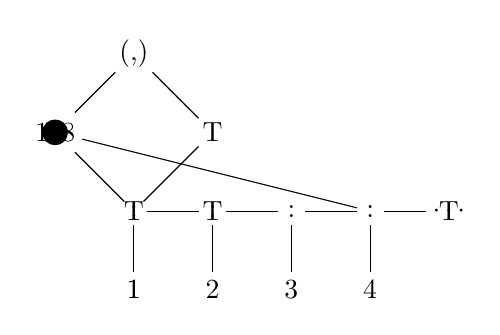
\begin{tikzpicture}
[level/.style={sibling distance=20mm/2^#1,level distance=6mm},
every node/.style={circle,inner sep=1.5pt},
eval/.style={circle,fill=black,color=black},
%every path/.style={->},
]
\path
  (0,0) node (comma) {(,)}
 +(-1,-1) coordinate (ct1)
 +(1,-1) coordinate (ct2)
 +(0,-2) coordinate (clt);
\onslide<1>{\node at (ct1) (t1) {T};}
\onslide<2-4>{\node[eval] at (ct1) (t1) {:};}
\onslide<5->{\node at (ct1) (t1) {1e8};}

\onslide<1->{\node at (ct2) (t2) {T};}

\onslide<1-2>{\node at (clt) (lt) {T};}
\onslide<3->{\node[alias=cons0] at (clt) (lt) {:};}
\onslide<3>{
	\path (cons0) +(0,-1) node (n) {1};
	\draw (cons0) -- (n);
	\path (cons0) +(1,0) node (cons1) {T};
	\draw (cons0) -- (cons1);
}
\onslide<4->{
	\onslide<4-6>{
	\path (cons0) +(0,-1) node (n) {1};
	\draw (cons0) -- (n);
	\path (cons0) +(1,0) node (cons1) {:};
	\draw (cons0) -- (cons1);

	\path (cons1) +(0,-1) node (n) {2};
	\draw (cons1) -- (n);
	\path (cons1) +(1,0) node (cons2) {:};
	\draw (cons1) -- (cons2);

	\path (cons2) +(0,-1) node (n) {3};
	\draw (cons2) -- (n);
	\path (cons2) +(1,0) node (cons3) {:};
	\draw (cons2) -- (cons3);
	}

	\path (cons3) +(0,-1) node (n) {4};
	\draw (cons3) -- (n);
	\onslide<4>{\path (cons3) +(1,0) node (cons4) {T};}
	\onslide<5->{\path (cons3) +(1,0) node (cons4) {$\cdots$};}
	\draw (cons3) -- (cons4);
	}
\draw (comma) -- (t1);
\draw (comma) -- (t2);
\onslide<1-3>{\draw (t1) -- (lt);}
\onslide<4>{\draw (t1) -- (cons3);}
\draw (t2) -- (lt);
\end{tikzpicture}
\end{center}
\end{frame}

\begin{frame}[fragile]
\frametitle{Source transformations may help}

\begin{haskell}
let xs () = [1..100000000]
in (last $ xs (), length $ xs ())
\end{haskell}
\vfill

\begin{center}
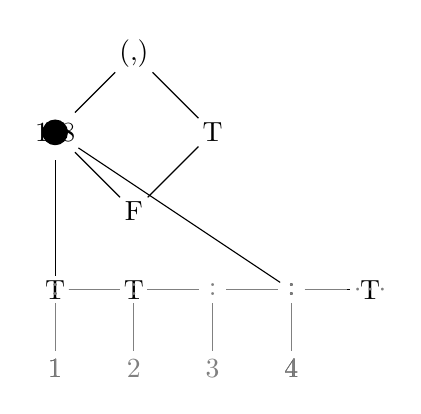
\begin{tikzpicture}
[level/.style={sibling distance=20mm/2^#1,level distance=6mm},
every node/.style={circle,inner sep=1.5pt},
eval/.style={circle,fill=black,color=black},
%every path/.style={->},
]
\path
  (0,0) node (comma) {(,)}
 +(-1,-1) coordinate (ct1)
 +(1,-1) coordinate (ct2)
 +(0,-2) coordinate (cf);
\onslide<1>{\node at (ct1) (t1) {T};}
\onslide<2-5>{\node[eval] at (ct1) (t1) {:};}
\onslide<6->{\node at (ct1) (t1) {1e8};}

\onslide<1->{\node at (ct2) (t2) {T};}

\onslide<1->{\node at (cf) (f) {F};}
\path (t1) +(0,-2) coordinate (clt);
\onslide<3>{\path (clt) node (lt) {T};}
\onslide<4>{\node[alias=cons0] at (clt) (lt) {:};}
\onslide<5-6>{\node[alias=cons0,color=gray] at (clt) (lt) {:};}
\onslide<4>{
	\path (cons0) +(0,-1) node (n) {1};
	\draw (cons0) -- (n);
	\path (cons0) +(1,0) node (cons1) {T};
	\draw (cons0) -- (cons1);
}
\onslide<5-6>{
	\begin{scope}[color=gray]
	\path (cons0) +(0,-1) node (n) {1};
	\draw (cons0) -- (n);
	\path (cons0) +(1,0) node (cons1) {:};
	\draw (cons0) -- (cons1);

	\path (cons1) +(0,-1) node (n) {2};
	\draw (cons1) -- (n);
	\path (cons1) +(1,0) node (cons2) {:};
	\draw (cons1) -- (cons2);

	\path (cons2) +(0,-1) node (n) {3};
	\draw (cons2) -- (n);
	\end{scope}

	\onslide<5>{
	\path (cons2) +(1,0) node (cons3) {:};
	\draw[color=gray] (cons2) -- (cons3);
	\path (cons3) +(0,-1) node (n) {4};
	\draw (cons3) -- (n);
	\path (cons3) +(1,0) node (cons4) {T};
	\draw (cons3) -- (cons4);
	}
	\onslide<6->{
	\begin{scope}[color=gray]
	\path (cons2) +(1,0) node (cons3) {:};
	\draw (cons2) -- (cons3);
	\path (cons3) +(0,-1) node (n) {4};
	\draw (cons3) -- (n);
	\path (cons3) +(1,0) node (cons4) {$\cdots$};
	\draw (cons3) -- (cons4);
	\end{scope}
	}
	}
\draw (comma) -- (t1);
\draw (comma) -- (t2);
\onslide<1-2>{\draw (t1) -- (f);}
\onslide<3-4>{\draw (t1) -- (lt);}
\onslide<5>{\draw (t1) -- (cons3);}
\draw (t2) -- (f);
\end{tikzpicture}

\vfill
\onslide<7->{(works, but fagile -- might be thwarted by compiler optimizations)}
\end{center}
\end{frame}

\begin{frame}[fragile]
\frametitle{Allow the programmer to copy a thunk: dup}

\begin{haskell}
let xs = [1..100000000]
in (case dup xs of Box xs' -> last xs',
    case dup xs of Box xs' -> length xs)
\end{haskell}
\vfill

\begin{center}
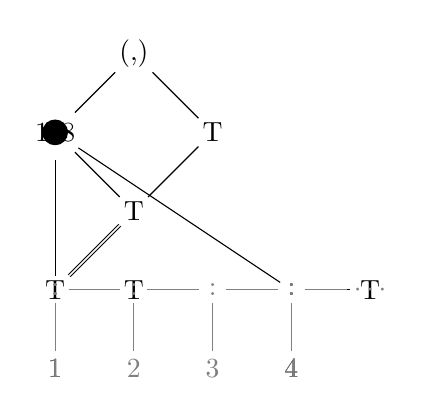
\begin{tikzpicture}
[level/.style={sibling distance=20mm/2^#1,level distance=6mm},
every node/.style={circle,inner sep=1.5pt},
eval/.style={circle,fill=black,color=black},
%every path/.style={->},
]
\path
  (0,0) node (comma) {(,)}
 +(-1,-1) coordinate (ct1)
 +(1,-1) coordinate (ct2)
 +(0,-2) coordinate (cot);
\onslide<1>{\node at (ct1) (t1) {T};}
\onslide<2-5>{\node[eval] at (ct1) (t1) {:};}
\onslide<6->{\node at (ct1) (t1) {1e8};}

\onslide<1->{\node at (ct2) (t2) {T};}

\onslide<1->{\node at (cot) (ot) {T};}
\path (t1) +(0,-2) coordinate (clt);
\onslide<3>{\path (clt) node (lt) {T};
	\draw[double] (lt) -- (ot);}
\onslide<4>{\node[alias=cons0] at (clt) (lt) {:};}
\onslide<5-6>{\node[alias=cons0,color=gray] at (clt) (lt) {:};}
\onslide<4>{
	\path (cons0) +(0,-1) node (n) {1};
	\draw (cons0) -- (n);
	\path (cons0) +(1,0) node (cons1) {T};
	\draw (cons0) -- (cons1);
}
\onslide<5-6>{
	\begin{scope}[color=gray]
	\path (cons0) +(0,-1) node (n) {1};
	\draw (cons0) -- (n);
	\path (cons0) +(1,0) node (cons1) {:};
	\draw (cons0) -- (cons1);

	\path (cons1) +(0,-1) node (n) {2};
	\draw (cons1) -- (n);
	\path (cons1) +(1,0) node (cons2) {:};
	\draw (cons1) -- (cons2);

	\path (cons2) +(0,-1) node (n) {3};
	\draw (cons2) -- (n);
	\end{scope}

	\onslide<5>{
	\path (cons2) +(1,0) node (cons3) {:};
	\draw[color=gray] (cons2) -- (cons3);
	\path (cons3) +(0,-1) node (n) {4};
	\draw (cons3) -- (n);
	\path (cons3) +(1,0) node (cons4) {T};
	\draw (cons3) -- (cons4);
	}
	\onslide<6>{
	\begin{scope}[color=gray]
	\path (cons2) +(1,0) node (cons3) {:};
	\draw (cons2) -- (cons3);
	\path (cons3) +(0,-1) node (n) {4};
	\draw (cons3) -- (n);
	\path (cons3) +(1,0) node (cons4) {$\cdots$};
	\draw (cons3) -- (cons4);
	\end{scope}
	}
	}
\draw (comma) -- (t1);
\draw (comma) -- (t2);
\onslide<1-2>{\draw (t1) -- (ot);}
\onslide<3-4>{\draw (t1) -- (lt);}
\onslide<5>{\draw (t1) -- (cons3);}
\draw (t2) -- (ot);
\end{tikzpicture}

\hide
\onslide<7->
consumer, not generator controls sharing\\
no code restructuring
\end{center}
\end{frame}

\newcommand{\mdup}{\text{\textsf{dup}}}
\newcommand{\mdeepDup}{\text{\textsf{deepDup}}}
\newcommand{\sVar}{\text{Var}}
\newcommand{\sExp}{\text{Exp}}
\newcommand{\sHeap}{\text{Heap}}
\newcommand{\sVal}{\text{Val}}
\newcommand{\sValue}{\text{Value}}
\newcommand{\sEnv}{\text{Env}}
\newcommand{\sApp}[2]{\operatorname{#1}#2}
\newcommand{\sLam}[2]{\text{\textlambda} #1.\, #2}
\newcommand{\sDup}[1]{\sApp \mdup #1}
\newcommand{\sDeepDup}[1]{\sApp \mdeepDup #1}
\newcommand{\sLet}[2]{\text{\textsf{let}}\ #1\ \text{\textsf{in}}\ #2}
\newcommand{\sred}[4]{#1 : #2 \Downarrow #3 : #4}
\newcommand{\sRule}[1]{\text{{\textsc{#1}}}}
\newcommand{\fv}[1]{\text{fv}(#1)}
\newcommand{\ufv}[1]{\text{ufv}(#1)}
\newcommand{\ur}[2]{\text{ur}_{#1}(#2)}
\newcommand{\dom}[1]{\text{dom}\,#1}
\newcommand{\fresh}[1]{#1'}


\begin{frame}
\frametitle{The sledgehammer: deepDup}

\begin{mathpar}
\inferrule
{\sred{\Gamma,x\mapsto e, \fresh x\mapsto \hat e} {\fresh x} \Delta z \\ \fresh x \text{ fresh}}
{\sred{\Gamma,x\mapsto e}{\sDup x} \Delta z}
\sRule{Dup}
\and
\inferrule
{
\sred{
\Gamma,
x\mapsto e,
\begin{array}[b]{l}
\fresh x\mapsto \hat e[\fresh y_1/y_1,\ldots, \fresh y_n/y_n],
\\
\fresh y_1 \mapsto \sDeepDup y_1,\ldots,
\fresh y_n \mapsto \sDeepDup y_n
\end{array}
} {\fresh x} \Delta z 
\\
\ufv e = \{y_1,\ldots,y_n\}
\\
\fresh x,\ \fresh y_1,\ldots,y_n \text{ fresh}
}
{\sred{\Gamma,x\mapsto e}{\sDeepDup x} \Delta z}
\sRule{Deep}
\end{mathpar}

\vfill
\begin{center}
\hide
morally, \lstinline-deepDup x- copies the whole heap reachable by x

\hide
\vfill
really, \lstinline-deepDup x- copies the whole heap reachable by x lazily
\end{center}

\end{frame}



\end{document}
